\documentclass[
	classe=$2^{de}$
]{coursclass}

\title{Chapitre 4 : Statistiques descriptives}
\author{}
\date{}

\begin{document}

\maketitle

\section{Proportions et pourcentages}

\begin{definition}[Population]
	\begin{itemize}
		\item Une \textbf{population} est un ensemble d'éléments, appelés les \textbf{individus}.
		\item Une \textbf{sous-population} est une partie de la population.
		\item Le nombre total d'individus dans la population est appelé l'\textbf{effectif total}.
	\end{itemize}
\end{definition}

\begin{remarque}
	Les individus d'une population ne sont pas toujours des personnes.

	Par exemple, on peut parler de la \textit{population} d'une trousse, dont les \textit{individus} sont les stylos, et une \textit{sous-population} est formée par les stylos rouges.
\end{remarque}

\begin{definition}[Proportion]
	On considère une population dont l'effectif total est $N$, et une sous-population dont l'effectif est $n$.
	\begin{itemize}
		\item La \textbf{proportion} d'individus dans la sous-population est $p = \dfrac{n}{N}$.
		\item On peut exprimer cette proportion en pourcentage, en la multipliant par $100$ :

		      $\left(\dfrac{n}{N}×100\right) \%$ des individus sont dans la sous-population.
	\end{itemize}
\end{definition}

\begin{exemple}
	\begin{center}
		\begin{tikzpicture}
			\foreach \x/\y in {0/0,0/1,1/0,1/1} {
					\node[red] at (\x,\y) {×};
				}
			\foreach \x/\y in {2/0,2/1,3/0,3/1,4/0,4/1} {
					\node at (\x,\y) {∙};
				}
		\end{tikzpicture}
	\end{center}
	Dans la population ci-dessus, la proportion de croix est $\dfrac{4}{10} = 0,4$, ou $40\%$.
\end{exemple}

\begin{remarque}
	Prendre $x\%$ d'une valeur revient à la multiplier par $\dfrac{x}{100}$.
\end{remarque}

\begin{propriete}[Proportion de proportion, pourcentage de pourcentage]
	\begin{center}
		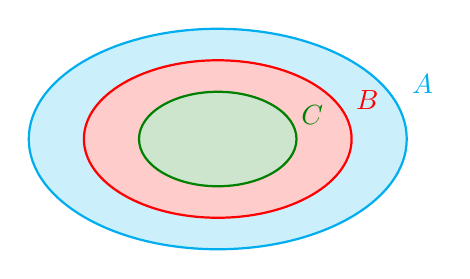
\begin{tikzpicture}
			\draw[thick,cyan,fill=cyan!20] (0,0) ellipse (2.4 and 1.4);
			\node[cyan] at (2.6,0.7) {$A$};
			\draw[thick,red,fill=red!20] (0,0) ellipse (1.7 and 1);
			\node[red] at (1.9,0.5) {$B$};
			\draw[thick,Green,fill=Green!20] (0,0) ellipse (1 and 0.6);
			\node[Green] at (1.2,0.3) {$C$};
		\end{tikzpicture}
	\end{center}

	On considère une population $A$, et
	\begin{itemize}
		\item Une sous-population $B$ de $A$, dont la proportion dans $A$ est $p_B$.
		\item Une sous-population $C$ de $B$, dont la proportion dans $B$ est $p_C$.
	\end{itemize}

	Alors la proportion de $C$ \uline{dans $A$} est $p = p_B × p_C$
\end{propriete}

\begin{exemple}
	On considère la population des véhicules possédés par une entreprise.

	\begin{itemize}
		\item $75\%$ de ces véhicules sont électriques.
		\item Parmi les véhicules électriques, $30\%$ sont des deux-roues.
	\end{itemize}
	La proportion $p$ de deux-roues électriques dans la population totale est donc
	$$ p = 0,75 × 0,3 = 0,225 $$
	Soit $22,5\%$.
\end{exemple}

\section{Variations et évolutions}
% TODO : pas trop long, ce n'est pas passionnant

\begin{definition}[Variations]
	Lorsqu'on passe d'une valeur $V₁$ à une valeur $V₂$, on dit qu'il s'agit d'une \textbf{évolution}. On a alors :
	\begin{itemize}
		\item $V₂ - V₁$ est la \textbf{variation absolue}.
		\item $\dfrac{V₂ - V₁}{V₁}$ est la \textbf{variation relative}, aussi appelée le \textbf{taux d'évolution}.
	\end{itemize}
\end{definition}

\begin{exemple}
	Une personne ayant $1\ 000\ 000$ d'euros gagne $1\ 000\ 000$ €.

	\begin{itemize}
		\item la variation absolue est de $1\ 000\ 000$ €.
		\item la variation relative est de $\dfrac{1\ 000\ 000}{100\ 000\ 000} = 0,01$, ou $1\%$.
	\end{itemize}
\end{exemple}

\begin{remarque}
	\begin{itemize}
		\item Si la variation absolue (ou le taux d'évolution) est positive, c'est que la valeur à augmenté. Sinon, c'est qu'elle a diminué.
		\item La variation absolue est dans la même unité que $V₁$ et $V₂$.
		\item Le taux d'évolution n'a pas d'unité.
	\end{itemize}
\end{remarque}

\begin{propriete}
	Si $t$ est le taux d'évolution entre deux valeurs $A$ et $B$, on a

	$$ B = A × (1 + t) $$
\end{propriete}
\begin{proof}
	On sait que $t$ est le taux d'évolution, donc $t = \dfrac{B - A}{A}$.

	Donc $A × t = B - A$, et donc
	$B = A × t + A = A × (1 + t)$.
\end{proof}

\begin{remarque}
	Si $t$ est \textit{supérieur à $0$}, c'est une augmentation. Sinon, c'est une diminution.
\end{remarque}

\begin{propriete}[Évolutions successives et coefficient global]
	Lorsqu'on applique plusieurs évolutions successives, on obtient le \textbf{coefficient global} en multipliant les coefficients.
\end{propriete}
\begin{exemple}
	Si on applique une augmentation de 20\%, suivie d'une diminution de 20\%, l'évolution a pour coefficient global
	$$ \left(1 + \frac{20}{100}\right) × \left(1 - \frac{20}{100}\right) = 1,2 × 0,8 = 0,96 $$
	On a donc globalement une diminution.
\end{exemple}

\begin{propriete}[Évolution réciproque]
	Si une évolution nous fait passer d'une valeur $A$ à une valeur $B$ en multipliant par $c$, on peut revenir à $A$ en \textit{divisant} par $c$.

	Cette nouvelle évolution est appelée \textbf{l'évolution réciproque}, et son coefficient est le \textbf{coefficient réciproque} $cᵣ = \frac{1}{c}$.
\end{propriete}

\begin{exemple}
	Si on passe de $150€$ à $240€$, on doit multiplier par $1,6$. \medskip

	Donc pour passer de $240€$ à $150€$, on doit multiplier par $\dfrac{1}{1,6} = 0,625$.
\end{exemple}

\section{Séries statistiques}

\begin{definition}[Moyenne, moyenne pondérée]
	Si on dispose d'une série de valeurs $x₁, ⋯, xₙ$,
	\begin{itemize}
		\item on peut calculer leur \textbf{moyenne} :
		      $$ M = \dfrac{x₁ + ⋯ + xₙ}{n} $$
		\item La moyenne peut être pondérée, c'est-à-dire que chaque valeur est multipliée par un coefficient $cᵢ$ :
		      $$ M = \dfrac{c₁ × x₁ + ⋯ + cₙ × xₙ}{c₁ + ⋯ + cₙ} $$
	\end{itemize}
\end{definition}

\begin{exemple}
	La moyenne de la série de notes $8 ; 11 ; 12 ; 17$ est
	$$ M = \dfrac{8 + 11 + 12 + 17}{4} = \dfrac{48}{4} = 12 $$

	Si la quatrième note (le $17$) était coefficient $2$, et que toutes les autres notes sont coefficient $1$, la moyenne devient
	$$ M = \dfrac{8 + 11 + 12 + 2 × 17}{1 + 1 + 1 + 2} = \dfrac{65}{5} = 13 $$
\end{exemple}

\begin{propriete}[Linéarité de la moyenne]
	\begin{itemize}
		\item Si on ajoute le même nombre $a$ à chaque valeur, la moyenne augmente de $a$.
		\item Si on multiplie chaque valeur par un nombre $b$, la moyenne est multipliée par $b$.
	\end{itemize}
\end{propriete}

\begin{definition}[Variance, écart-type]
	Si on dispose d'une série de valeurs $x₁, ⋯, xₙ$, et qu'on dispose de la moyenne $M$, on définit
	\begin{itemize}
		\item La \textbf{variance} de cette série
		      $$ V = \dfrac{(x₁ - M)² + ⋯ + (xₙ - M)²}{n} $$
		\item L'\textbf{écart-type} de cette série
		      $$ σ = \sqrt{V} $$
	\end{itemize}
\end{definition}

\begin{exemple}
	Prenons la série de notes $1 ; 4 ; 9 ; 15 ; 18 ; 13$.

	La moyenne de cette série est $10$. Donc on a
	\begin{itemize}
		\item $V = \dfrac{(1 - 10)² + (4 - 10)² + (9 - 10)² + (15 - 10)² + (18 - 10)² + (13 - 10)²}{6}$ \vspace{0.5em}

		      $\phantom{V} = \dfrac{(-9)² + (-6)² + (-1)² + 5² + 8² + 3²}{6}$ \vspace{0.5em}

		      $\phantom{V} = \dfrac{81 + 36 + 1 + 25 + 64 + 9}{6}$ \vspace{0.5em}

		      $\phantom{V} = \dfrac{216}{6} = 36$
		\item $σ = \sqrt{V} = \sqrt{36} = 6$
	\end{itemize}
\end{exemple}

\end{document}